Da die Minispiele alle einem ähnlichen Grundaufbau folgen, bietet es sich an, diesen objektorientiert und modular zu implementieren, um Redundanz zu vermeiden.
Dieser Grundaufbau besteht aus folgenden Klassen:

\begin{itemize}
    \item \texttt{LevelScene}
    \item \texttt{LevelSelectorScene}
    \item \texttt{MinigameEndScene}
    \item \texttt{Minigames}
\end{itemize}

\paragraph{LevelScene} Diese abstrakte Klasse ist eine Erweiterung der \texttt{BaseScene} und stellt Fachschaft übergreifende Variablen und Methoden zur Verfügung.
Sie beinhaltet:

\begin{sloppypar}
    \begin{itemize}
        \item \texttt{REWARD}: Ein \texttt{ItemObject}, welches die Spielen nach erfolgreichendem Beenden des Levels erhalten.
            Es wird mit Hilfe der Funktion \texttt{getMinigameReward} der \texttt{ItemObject}-Klasse generiert.
        \item Ein \texttt{BackdropObject} welches das zur Fachschaft gehörende Hintergrundbild beinhaltet.
        \item \texttt{exitButton}: Ein \texttt{ButtonObject}, welches das Verlassen des Minispiels mittels Entfernung der obersten zwei Scenen des \texttt{SceneStack} (\texttt{LevelScene} und \texttt{LevelSelectorScene}) ermöglicht.
        \item \texttt{menuButton}: Ein \texttt{ButtonObject}, welches die Rückkehr zur Level-Auswahl mittels Entfernung der obersten Scene des \texttt{SceneStack} (\texttt{LevelScene}) ermöglicht.
        \item \texttt{reset()}: Eine abstrakte Funktion, welche das Zurücksetzten eines Levels ermöglichen soll.
            Dafür wird sie von den Leveln der Fachschaften implementiert, welche dann je nach Minispiel eine komplett neue Instanz erstellen, oder nur einzelne Elemente neu generieren.
        \item \texttt{levelWon()}: Eine Prozedur, wodurch eine Instanz der \texttt{MinigameEndScene} auf den \texttt{SceneStack} gepushed wird und \texttt{REWARD} in das Inventar der Spielfigur übergeben wird.
        \item \texttt{levelLost()}: Eine Prozedur, wodurch eine Instanz der \texttt{MinigameEndScene} auf den \texttt{SceneStack} gepushed wird.
        \item \texttt{LevelScene(Department department, int level)}: Der Konstruktor der Klasse, welcher mit Hilfe seiner Parameter das Hintergrundbild lädt und die Knöpfe platziert.
    \end{itemize}
\end{sloppypar}

\paragraph{LevelSelectorScene} Diese Klasse ist eine Erweiterung der \texttt{BaseScene} und verknüpft, neben anderen Funktionen, jeweils drei \texttt{LevelScenes} miteinander.
Sie beinhaltet:

\begin{sloppypar}
    \begin{itemize}
        \item \texttt{LEVELS}: Ein \texttt{LevelScene}-Array, welches die drei Level beinhaltet.
        \item Ein \texttt{BackdropObject} welches das Hintergrundbild beinhaltet.
        \item \texttt{exitButton}: Ein \texttt{ButtonObject}, welches das Verlassen des Minispiels mittels Entfernung der obersten Scene des \texttt{SceneStack} (\texttt{LevelSelectorScene}) ermöglicht.
        \item \texttt{buttonLevel1}: Ein \texttt{ButtonObject}, welches die erste in \texttt{LEVELS} gespeicherte \texttt{LevelScene} auf den \texttt{SceneStack} pushed.
        \item \texttt{buttonLevel2}: Ein \texttt{ButtonObject}, welches die zweite in \texttt{LEVELS} gespeicherte \texttt{LevelScene} auf den \texttt{SceneStack} pushed.
        \item \texttt{buttonLevel3}: Ein \texttt{ButtonObject}, welches die dritte in \texttt{LEVELS} gespeicherte \texttt{LevelScene} auf den \texttt{SceneStack} pushed.
        \item \texttt{LevelSelectorScene(LevelScene level1, LevelScene level2, LevelScene level3)}: Der Konstruktor der Klasse, welcher mit Hilfe seiner Parameter das Hintergrundbild lädt und die Knöpfe platziert.
    \end{itemize}
\end{sloppypar}

\paragraph{MinigameEndScene} Diese Klasse ist eine Erweiterung der \texttt{BaseScene} und ist für das Ende eines Levels zuständig.
Sie beinhaltet:

\begin{sloppypar}
    \begin{itemize}
        \item Ein \texttt{BackdropObject} welches einen schwarzen, semi-transparenten Hintergrund beinhaltet, um das Level zu verdunkeln.
        \item \texttt{banner}: Ein \texttt{BaseObject}, welches entweder den Schriftzug \glqq GEWONNEN\grqq{} oder \glqq VERLOREN\grqq{} darstellt.
        \item \texttt{rewardContainer}: Ein \texttt{BaseObject}, welches als Rahmen für das gewonnene Item dient.
            Es wird nur gezeichnet, falls das Level gewonnen wurde.
        \item \texttt{rewardItem}: Ein \texttt{BaseObject}, welches das gewonnene Item darstellt.
            Es wird nur gezeichnet, falls das Level gewonnen wurde.
        \item \texttt{exitButton}: Ein \texttt{ButtonObject}, welches das Level mittels der Prozedur \texttt{resetMinigameLevel} der \texttt{Minigames}-Klasse, auf die später noch einmal eingengangen wird, ohne es direkt neu zu starten zurücksetzt und das Minispiel mittels Entfernung der obersten Scene des \texttt{SceneStack} (nach Zurücksetzen: \texttt{LevelSelectorScene}) verlässt.
        \item \texttt{menuButton}: Ein \texttt{ButtonObject}, welches das Level mittels der Prozedur \texttt{resetMinigameLevel} der \texttt{Minigames}-Klasse ohne es direkt neu zu starten zurücksetzt..
        \item \texttt{retryButton}: Ein \texttt{ButtonObject}, welches das Level mittels der Prozedur \texttt{resetMinigameLevel} der \texttt{Minigames}-Klasse zurücksetzt.
        \item \texttt{MinigameEndScene(boolean won, int level, ItemObject reward)}: Der Konstruktor der Klasse, welcher mit Hilfe seiner Parameter das Hintergrundbild, das Banner und gegebenenfalls die Belohnung lädt, sowie die Knöpfe platziert.
    \end{itemize}
\end{sloppypar}

\paragraph{Minigames} Diese Klasse ist statisch und stellt Methoden zum Starten und Zurücksetzen der Minispiele zur Verfügung.
Sie beinhaltet:

\begin{sloppypar}
    \begin{itemize}
        \item \texttt{generateMinigame(Department department)}: Eine Funktion, welche abhängig von der als Parameter gegebenen Fachschaft eine \texttt{LevelSelectorScene} mit den passenden Leveln zurückgibt.
        \item \texttt{resetMinigameLevel(int level, boolean autoRetry)}: Eine Prozedur, welche die obersten zwei Scene des \texttt{SceneStack} (\texttt{MinigameEndScene} und \texttt{LevelScene}, da diese Funktion nur nach dem Beenden eines Minispieles aufgerufen wird) entfernt und das als Parameter gegebene Level der jetzt oben liegenden \texttt{LevelSelectorScene} mittels der \texttt{reset}-Funktion des Levels zurücksetzt.
            Falls der Parameter \texttt{autoRetry} wahr ist, wird zusätzlich das zurückgesetzte Level auf den \texttt{SceneStack} gepushed.
        \item \texttt{Minigames}: Der Konstruktor der Klasse, welcher als \texttt{private} deklariet ist, da er nicht aufgerufen werden soll.
    \end{itemize}
\end{sloppypar}

Um also ein Minispiel für eine Fachschaft zu implementieren müssen folgende Dinge geschehen:


\begin{sloppypar}
    \begin{enumerate}
        \item Erweiterung der \texttt{LevelScene}, um die Funktionsweise des Spieles zu implementieren.
        \item Hinzufügen von weiteren Klassen oder Resourcen, die von der erweiterten \texttt{LevelScene} benötigt werden.
        \item Hinzufügen eines \texttt{ButtonObject} in der, den Raum der Fachschaft repräsentierenden, Scene (beispielsweise \texttt{MatheraumScene}), welcher die von \texttt{Mingames.generateMinigame} erstellte \texttt{LevelSelectorScene} auf den \texttt{SceneStack} pushed.
    \end{enumerate}
\end{sloppypar}

In den folgenden Abschnitten sind diese fachschaftspezifischen Erweiterungen erklärt.

\subsubsection{Informatik}

\begin{sloppypar}
    Für das Minispiel der Fachschaft Informatik wurde die \texttt{LevelScene} zur \texttt{ComputerScienceLevelScene} erweitert, um das Zeichnen, Auswählen und Überprüfen der Logikgatter, sowie das Zeichnen des Schaltkreises zu ermöglichen.
    Außerdem wird ein \texttt{LogicGate}-Enum, welches die Gatter verwaltet, sowie ein \texttt{ComputerSciencePuzzle}-Enum, das die Schaltkreise bereit stellt, hinzugefügt.    
\end{sloppypar}

\paragraph{LogicGate} Die Implementierung mittels einer Enumeration bietet sich an, da vorgegebene Logikgatter definiert werden, die nicht verändert oder durch weitere ergänzt werden können.
Jede Enum-Konstante speichert zusätzlich noch ein Bild, welches das Gatter repräsentiert.
Zusätzlich werden noch Funktionen zur Generierung einer zufälligen Auswahl an Logikgattern, welche als Antwortmöglichkeiten fungieren, implementiert.
Sie beinhaltet:

\begin{sloppypar}
    \begin{itemize}
        \item \texttt{SPRITE}: Ein \texttt{java.awt.Image}, das das zum Logikgatter gehörende Bild speichert.
        \item \texttt{getRandom()}: Eine Funktion, welche eine zufällige Enum-Konstante mittels der \texttt{java.util.Random}-Klasse zurückgibt.
        \item \texttt{getRandomArray(int length, LogicGate[] includedGates)}: Eine Funktion, welche ein zufällig generiertes Array an Enum-Konstanten der Länge \texttt{length} zurückgibt, welches jedes Gatter höchstens einmal und alle in \texttt{includedGates} gegebenen Gatter enthält. 
        \item \texttt{LogicGate(String path)}: Der Konstruktor der Klasse, welcher nur von der Klasse selbst bei der Initialisierung der Konstanten aufgerufen wird.
            Er speichert das durch \texttt{path} gegebene Bild in \texttt{SPRITE}.
    \end{itemize}
\end{sloppypar}

Die \texttt{getRandomArray}-Methode ist zur näheren Erklärung im Folgenden dargestellt.

\begin{lstlisting}[caption=getRandomArray-Methode, label=lst:mggetRandomArray, captionpos=t, language=Java]
public static LogicGate[] getRandomArray(
    int length, LogicGate[] includedGates
) {
    // Das zu generierende Array
    LogicGate[] out = new LogicGate[length];
    // Indizes der Gatter, die beinhaltet werden sollen
    List<Integer> includedGatesIdx = new ArrayList<>();

    // Abbruch, falls mehr Gatter zurückgegeben werden sollen,
    // als Enum-Konstanten existieren.
    if (length > LogicGate.values().length) return null;

    // Abbruch, falls die Länge der zu beinhaltenden Gatter
    // größer ist, als die der gesamten Liste.
    if (includedGates.length > length) return null;

    // Generierung der Indizes der Gatter, die beinhaltet
    // werden sollen
    for (int i = 0; i < includedGates.length; i++) {
        // zufälliger Index
        int r = new Random().nextInt(length);

        // Neuer zufälliger Index, solange der alte bereits
        // generiert wurde
        while (includedGatesIdx.contains(r)) {
            r = new Random().nextInt(length);
        }

        // Hinzufügen des Indexes
        includedGatesIdx.add(r);
    }

    // Generierung des Logikgatter-Arrays
    for (int i = 0; i < length; i++) {
        // Überprüfung, ob an Index i ein gegebenes Gatter
        // platziert oder ein neues Gatter generiert werden soll
        if (includedGatesIdx.contains(i)) {
            // Hinzufügen des gegebenen Gatters an dem
            // in includedGatesIdx gespeicherten Index
            out[i] = includedGates[includedGatesIdx.indexOf(i)];
        } else {
            // Zufälliges Gatter
            LogicGate rGate = getRandom();
            // Neues zufälliges Gatter, solange das alte
            // entweder in den gegebenen Gattern oder
            // in dem bereits generierten Array enthalten ist.
            while (
                Arrays.asList(includedGates).contains(rGate) ||
                Arrays.asList(out).contains(rGate)
            ) {
                rGate = getRandom();
            }

            // Hinzufügen des Gatters
            out[i] = rGate;
        }
    }

    // Rückgabe des fertigen Arrays
    return out;
}
\end{lstlisting}

\paragraph{ComputerSciencePuzzle} Die Implementierung mittels einer Enumeration bietet sich an, da vorgegebene Schaltkreise definiert werden, die nicht verändert oder durch weitere ergänzt werden können.
Sie beinhaltet:

\begin{sloppypar}
    \begin{itemize}
        \item \texttt{PUZZLES}: Ein statisches, zweidimensionales \texttt{ComputerSciencePuzzle}-Array, welches für jedes Level die zugehörigen Enum-Konstanten speichert.
        \item \texttt{SPRITE}: Ein \texttt{java.awt.Image}, das das zum Puzzle gehörende Bild speichert.
        \item \texttt{SOLUTION}: Ein \texttt{LogicGate}-Array, das die im Schaltkreis abgedeckten Logikgatter enthält.
        \item \texttt{ANSWERS}: Ein \texttt{LogicGate}-Array, das die zur Auswahl stehenden Antwortmöglichkeiten beinhaltet.
        \item \texttt{getPuzzle(int level)}: Eine Funktion, welche eine zufällige Enum-Konstante basierend auf dem gegebenen level, mittels der \texttt{java.util.Random}-Klasse zurückgibt.
        \item \texttt{ComputerSciencePuzzle(String path, LogicGate[] solution, int amountOfAnswers)}: Der Konstruktor der Klasse, welcher nur von der Klasse selbst bei der Initialisierung der Konstanten aufgerufen wird.
            Er speichert das durch \texttt{path} gegebene Bild in \texttt{SPRITE}, die Lösung \texttt{solution} in \texttt{SOLUTION} und generiert \texttt{ANSWERS} mittels \texttt{LogicGate.getRandomArray}.
    \end{itemize}
\end{sloppypar}

\paragraph{ComputerScienceLevelScene} Eine erweiterung der \texttt{LevelScene}, welche die grundlegenden Methoden des Informatik-Minispieles implementiert.
Sie beinhaltet:

\begin{sloppypar}
    \begin{itemize}
        \item \texttt{LEVEL}: Die ID des Levels.
        \item \texttt{PUZZLE}: Das \texttt{ComputerSciencePuzzle} des Levels.
        \item \texttt{ANSWER\_FRAMES}: Ein \texttt{BaseObject}-Array, das die Rahmen enthält, die um ausgewählte Antworten gezeichnet werden.
        \item \texttt{ACTIVE\_ANSWERS}: Ein \texttt{LogicGate}-Array, das die geantworteten Logikgatter enthält.
        \item \texttt{setAnswer(LogicGate gate, int x, int y)}: Eine Prozedur, welche für das Antworten verantwortlich ist.
            Sie setzt die Rahmen, aktualisiert die geantworteten Gatter, überprüft ob eine Lösung richtig oder falsch ist und beendet das Minispiel entsprechend.
        \item \texttt{reset()}: Eine Funktion, die die \texttt{reset}-Methode der \texttt{LevelScene} implementiert, indem sie eine neu generierte \texttt{ComputerScienceLevelScene} zurückgibt.
        \item \texttt{ComputerScienceLevelScene(int level)}: Der Konstruktor der Klasse, welcher alle Variablen initialisiet und die Gatter, sowie den Schaltkreis platziert.
    \end{itemize}
\end{sloppypar}

Die \texttt{setAnswer}-Methode ist zur näheren Erklärung im Folgenden als Struktogramm dargestellt.

\begin{figure}[H]
	\centering
	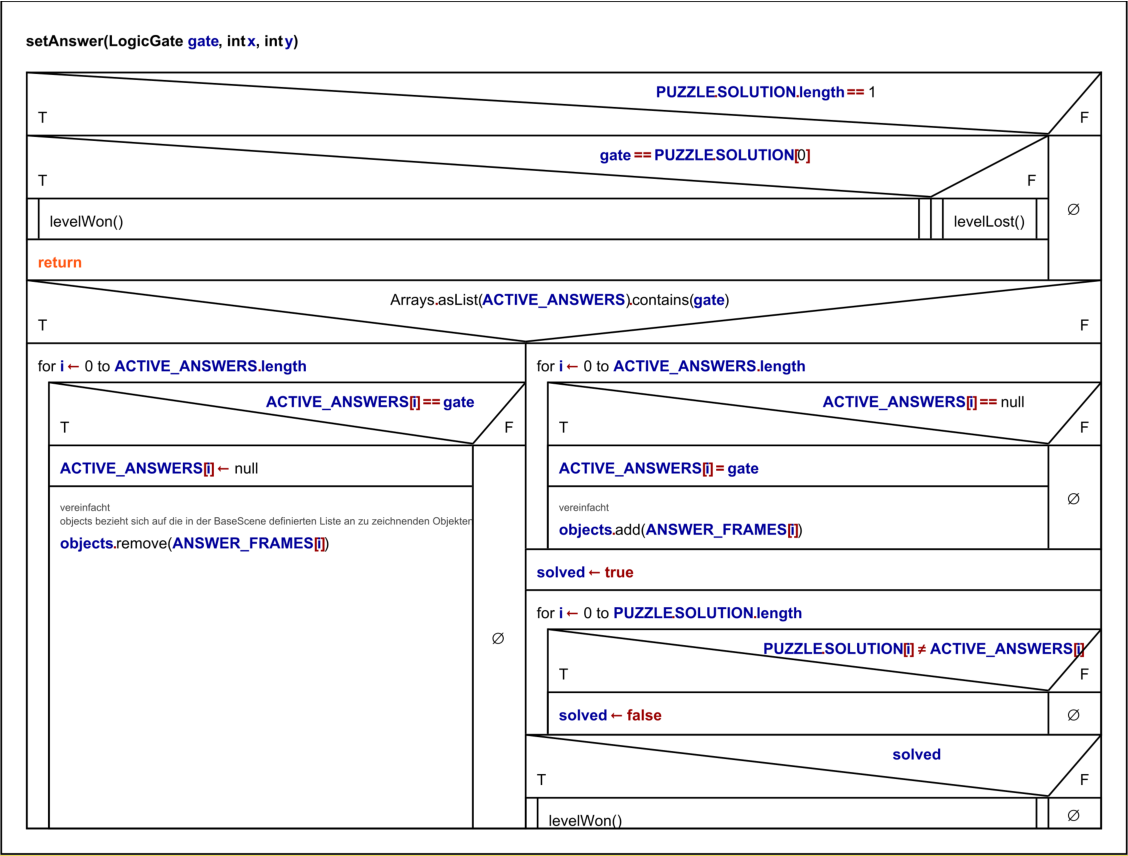
\includegraphics[width=1\textwidth]{bilder/StruktogrammSetAnswer.pdf}
	\caption{Struktogramm der setAnswer-Methode}
	\label{fig:mgsetAnswer}
\end{figure}

\subsubsection{Mathematik}

\begin{sloppypar}
    Für das Minispiel der Fachschaft Mathematik wurde die \texttt{LevelScene} zur \texttt{MathematicsLevelScene} erweitert, um das Zeichnen und Überprüfen der Tangramsteine, sowie das Zeichnen der Silhouette zu ermöglichen.
    Außerdem wird eine \texttt{TangramPieceObject}-Klasse, welche die Tangramsteine verwaltet, sowie ein \texttt{MathematicsPuzzle}-Enum, das die Silhouette bereit stellt, hinzugefügt.    
\end{sloppypar}

\paragraph{TangramPieceObject} Diese Klasse erweiter das \texttt{BaseObject}.
Dadurch sorgt sie dafür, dass jeder Stein ein Bild besitzt und verschoben, sowie rotiert werden kann.
Sie beinhaltet:

\begin{sloppypar}
    \begin{itemize}
        \item \texttt{SPRITE\_PATH}: Der Pfad zum Bild des Steines.
        \item \texttt{originalWidth, originalHeight}: Die Ausgangsgröße des Steines.
        \item \texttt{rotation}: Die Rotation des Steines.
        \item \texttt{levelScene}: Die \texttt{MathematicsLevelScene}, zu der der Stein gehört.
        \item \texttt{isDragged}: Ein \texttt{boolean}, welcher speichert, ob der Stein gerade gezogen wird.
        \item \texttt{generatePieces()}: Eine statische Funktion, die ein Array, welches alle Tangram Steine beinhaltet, zurückgibt.
        \item \texttt{setLevelScene(TangramPieceObject[] pieces, MathematicsLevelScene levelScene)}: Eine statische Prozedur, die bei jedem in \texttt{pieces} gegebenen Tangram-Stein die \texttt{levelScene} festlegt.
        \item \texttt{rotate(double degree)}: Eine Prozedur, die den Stein um den gegebenen Winkel in mathematisch negative Richtung dreht.
        \item \texttt{setRotation(double degree)}: Eine Prozedur, die den Stein so dreht, dass dieser eine Rotation von \texttt{degree} besitzt.
        \item \texttt{update(BaseScene scene)}: Eine Implementierung der \texttt{update}-Prozedur der \texttt{BaseScene}.
            Sie ermöglicht Verschiebung und Drehung des Tangram-Steines.
        \item \texttt{TangramPieceObject(int id)}: Der Konstruktor der Klasse, welcher als \texttt{private} deklariert ist, da immer ein gesamter Satz Tangram-Steine mittels der \texttt{generatePieces}-Funktion erstellt werden soll.
            Er lädt das von \texttt{id} abhängige Bild und initialisiert Variablen.
    \end{itemize}
\end{sloppypar}

Die \texttt{update}-Methode ist zur näheren Erklärung im Folgenden dargestellt.

\begin{lstlisting}[caption=update-Methode des TangramPieceObject, label=lst:mggetRandomArray, captionpos=t, language=Java]
public void update(BaseScene scene) {
    // Aktuelle und vorherige Maus-Position abfragen
    Point mousePos = Input.INSTANCE.getMousePosition();
    Point lastMousePos = Input.INSTANCE.getLastMousePosition();
    // Diese *können* (technisch gesehen) null sein
    if(mousePos == null || lastMousePos == null)
        return;

    if (!isDragged && !levelScene.isDragging && isClicked(false)) {
        // Wenn das Objekt angeklickt wird und noch kein Stein
        // gezogen wird, verschieben wir es an oberste Stelle
        // (z-Achse) und beginnen, es zu ziehen
        scene.objects.remove(this);
        scene.objects.add(this);

        isDragged = true;

        // Außerdem teilen wir der levelScene mit,
        // dass jetzt ein Stein gezogen wird
        levelScene.isDragging = true;
    } else if (isDragged && !Input.INSTANCE.getMouseState(MouseEvent.BUTTON1).isDown()) {
        // Wenn die linke Maustaste losgelassen wird,
        // wird das Objekt nicht mehr gezogen,
        isDragged = false;
        // Der levelScene mitgeteilt,
        // dass kein Stein mehr gezogen wird
        levelScene.isDragging = false;
        // Und überprüft, ob das Puzzle gelöst ist
        levelScene.checkPuzzle();
    }

    if (isDragged) {
        // Berechnung der neuen Position
        int newPosX = x + mousePos.x - lastMousePos.x;
        int newPosY = y + mousePos.y - lastMousePos.y;
        // Überprüfung, ob die neue Position innerhalb
        // des Bildschirms liegt
        if (
            newPosX > 0 && newPosX + width < MainWindow.WIDTH &&
            newPosY > 0 && newPosY + height < MainWindow.HEIGHT
        ) {
            // Aktualisierung der Position
            x = newPosX;
            y = newPosY;
        }

        // Rotieren des Objektes, falls 'R' gedrückt wird
        if(
            Input.INSTANCE.getKeyState(KeyEvent.VK_R) ==
            Input.KeyState.PRESSED
        ) {
            rotate(45);
        }
    }
}
\end{lstlisting}

\paragraph{MathematicsPuzzle} Die Implementierung mittels einer Enumeration bietet sich an, da vorgegebene Silhouetten definiert werden, die nicht verändert oder durch weitere ergänzt werden können.
Sie beinhaltet:

\begin{sloppypar}
    \begin{itemize}
        \item \texttt{PUZZLES}: Ein statisches, zweidimensionales \texttt{MathematicsPuzzle}-Array, welches für jedes Level die zugehörigen Enum-Konstanten speichert.
        \item \texttt{SPRITE}: Ein \texttt{java.awt.Image}, das das zum Puzzle gehörende Bild speichert.
        \item \texttt{MARGIN\_OF\_ERROR}: Die prozentuale Abweichung der bedeckten Fläche, sodass eine Belegung trotzdem als Lösung gilt.
        \item \texttt{SOLUTIONS}: Ein dreidimensionales \texttt{Double}-Array, welches für jede Lösung (erste Dimension), für jeden Tangram-Stein (zweite Dimension) die X-Position, Y-Position und Rotation (dritte Dimension) speichert.
            Dabei werden erstere als relative Position gespeichert, also als \texttt{double} zwischen $0$ und $1$, der angibt, bei wie viel Prozent der Gesamtbreite beziehungsweise Gesamthöhe sich der Stein befindet.
            Eine Besonderheit stellt der Ausgangszustand, welcher ebenfalls als ein Puzzle gespeichert wird, bei dem alle Steine vorgegeben sind, dar.
            Dieser speichert zusätzlich noch die Breite und die Höhe der Steine, um diese entsprechend zurückzusetzten.
            Wichtig ist, dass diese Lösungen nur zum Vorgeben der Tangramsteine verwendet werden und nicht zur Überprüfung einer Belegung dieser.
            Dadurch ist es auch nicht unbedingt notwendig mehrere Lösungen pro Puzzle zu definieren, jedoch entsteht dadurch mehr Variabilität.
        \item \texttt{AMOUNT\_OF\_GIVEN\_PIECES}: Die Anzahl an bereits platzierten Steinen.
        \item \texttt{ANSWERS}: Ein \texttt{LogicGate}-Array, das die zur Auswahl stehenden Antwortmöglichkeiten beinhaltet.
        \item \texttt{getPuzzle(int level)}: Eine Funktion, welche eine zufällige Enum-Konstante basierend auf dem gegebenen level, mittels der \texttt{java.util.Random}-Klasse zurückgibt.
        \item \texttt{isSolutionValid(int x, int y, int width)}: Eine Funktion, die berechnet, wie viele Pixel der Silhouette von Tangramsteinen verdeckt sind und wie viele Pixel die Silhouette insgesamt enthält.
            Dadurch wird dann ermittelt, wie viel Prozent der Silhoutte verdeckt sind und $p\% < 1-MARGIN\_OF\_ERROR$ zurückgegeben.
        \item \texttt{setGivenPieces(TangramPieceObject[] pieces, int x, int y, int width, int height)}: Eine Prozedur, die die richtige Position und Rotation zufällig aus \texttt{pieces} ausgewählter Tangramsteine vorgibt.
        \item \texttt{reset(TangramPieceObject[] pieces, int x, int y, int size, int px, int py, int pwidth, int pheight)}: Eine Prozedur, welche die Steine mittels \texttt{setGivenPieces} in den Ausgangszustand zurücksetzt und neu für das Puzzle vorgibt.
        \item \texttt{MathematicsPuzzle(String path, int amountOfGivenPieces, double[][][] solutions)}: Der Konstruktor der Klasse, welcher nur von der Klasse selbst bei der Initialisierung der Konstanten aufgerufen wird.
            Er initialisiert die Variablen mit den durch die Parameter gegebenen Werten.
    \end{itemize}
\end{sloppypar}

Die \texttt{setGivenPieces}-Methode ist zur näheren Erklärung im Folgenden dargestellt.
Da sie teilweise stark der im Programmcode \ref{lst:mggetRandomArray} abgebildeten Methode ähnelt wurde sie verkürzt dargestellt.

\begin{lstlisting}[caption=update-Methode des TangramPieceObject, label=lst:mggetRandomArray, captionpos=t, language=Java]
private void setGivenPieces(
    TangramPieceObject[] pieces, int x, int y, int width, int height
) {
    // Generierung der zufälligen Indizes der vorzugebenden Steine
    int[] idx = new int[AMOUNT_OF_GIVEN_PIECES];
    
    [ausgelassen]

    // Festlegen einer Lösung des Puzzles
    int rSolution = new Random().nextInt(SOLUTIONS.length);
    // Positionierung der Steine
    for(int i : idx) {
        // Rotation wird als erstes geändert, da sich dadurch
        // die Größe und somit die Position des Steines ändern kann.
        pieces[i].setRotation(SOLUTIONS[rSolution][i][2]);
        pieces[i].x = (int) (x + SOLUTIONS[rSolution][i][0]*width);
        pieces[i].y = (int) (y + SOLUTIONS[rSolution][i][1]*height);

        // Höhe und Breite der Steine zurücksetzten,
        // falls es sich beim Puzzle um den Ausgangszustand handelt
        if(this == P_INIT) {
            pieces[i].width =
            (int) (SOLUTIONS[rSolution][i][3]*width);
            pieces[i].height =
            (int) (SOLUTIONS[rSolution][i][4]*height);
            pieces[i].originalWidth = pieces[i].width;
            pieces[i].originalHeight = pieces[i].height;
        }
    }
}
\end{lstlisting}

\paragraph{MathematicsLevelScene} Eine erweiterung der \texttt{LevelScene}, welche die grundlegenden Methoden des Mathematik-Minispieles implementiert.
Sie beinhaltet:

\begin{sloppypar}
    \begin{itemize}
        \item \texttt{PIECES}: Ein \texttt{TangramPieceObject}-Array, welches die Tangramsteine des Levels speichert.
        \item \texttt{PUZZLE}: Das \texttt{MathematicsPuzzle} des Levels.
        \item \texttt{PUZZLE\_X}: Die X-Position der Silhouette.
        \item \texttt{PUZZLE\_Y}: Die Y-Position der Silhouette.
        \item \texttt{PUZZLE\_WIDTH}: Die Breite der Silhouette.
        \item \texttt{PUZZLE\_HEIGHT}: Die Höhe der Silhouette.
        \item \texttt{isDragging}: Ein \texttt{boolean}, der speichert, ob gerade ein Tangramstein gezogen wird.
            Dadurch wird verhindert, dass mehrere Steine gleichzeitig gezogen werden.
        \item \texttt{reset()}: Eine Funktion, die die \texttt{reset}-Methode der \texttt{LevelScene} implementiert, indem sie eine neu generierte \texttt{MathematicsLevelScene} zurückgibt.
        \item \texttt{checkPuzzle()}: Eine Prozedur, die mittels der \texttt{isSolutionValid}-Methode des \texttt{PUZZLE} überprüft, ob das Level gelöst wurde und in diesem Fall das Level beendet.
        \item \texttt{MathematicsLevelScene(int level)}: Der Konstruktor der Klasse, welcher alle Variablen initialisiet und die Steine, sowie die Silhouette platziert.
    \end{itemize}
\end{sloppypar}